\documentclass[letterpaper,11pt]{article}
\usepackage{graphicx}
\usepackage{listings}
\usepackage[super]{nth}
\usepackage[hyphens]{url}
\usepackage{hyperref}
\usepackage{amsmath}
\usepackage[makeroom]{cancel}
\usepackage[table]{xcolor}
\usepackage{comment}
\usepackage[space]{grffile}
\usepackage{csvsimple}
\usepackage{longtable}
\usepackage{adjustbox}


\newcommand*{\srcPath}{../src}%

\lstset{
	basicstyle=\footnotesize,
	breaklines=true,
}

\begin{document}

\begin{titlepage}

\begin{center}

\Huge{Assignment 9}

\Large{CS 532:  Introduction to Web Science}

\Large{Spring 2018}

\Large{Hrishi Gadkari}


\end{center}

\end{titlepage}

\newpage


% =================================
% First question
% =================================
\section*{1}

\subsection*{Question}

\begin{verbatim}
1.  Using the data from A7:

- Consider each row in the blog-term matrix as a 1000 dimension vector, 
corresponding to a blog.  

- Use knnestimate() to compute the nearest neighbors for both:
	http://f-measure.blogspot.com/
	http://ws-dl.blogspot.com/

	for k={1,2,5,10,20}.

	Use cosine distance metric (chapter 8) not euclidean distance. 
	So you have to implement numpredict.cosine() instead of using 
	numpredict.euclidean() in:
	https://github.com/arthur-e/Programming-Collective-Intelligence/blob/master/
	chapter8/numpredict.py

\end{verbatim}

\clearpage
\subsection*{Answer}

Since I had not done Assignment 7, I decided to use \textbf{blogdata.txt} from one my classmatesv\cite{gitref} github account. I then modified the \textbf{numpredict.py} as memtioned in the question \cite{numref} for the functions knnestimate, getdistances and cosine. In knnestimate I removed the average value whereas I implemented cosine similarity using scipy library \cite{libref}. For the getdistance, I removed the Euclidean distance function and used cosine function instead. The changes looks as follows:

\lstinputlisting[firstline=38,lastline=79,frame=single,caption={Python program for modifies numpredict.py},label=lst:q1nump,captionpos=b,numbers=left,showspaces=false,showstringspaces=false,basicstyle=\footnotesize]{numpredict.py}

In-order to get the vector data from \textbf{blogdata.txt}, I fetched the blogdata in tuples and added to specified blog arrays and created new dictionary with blog as key. I have placed the program in \textbf{knncalc.py}. The vectors were then used for the cosine measurement by running through the F-measure and WSDL group blogs.

\lstinputlisting[frame=single,caption={Python program for KNN},label=lst:q1knncalc,captionpos=b,numbers=left,showspaces=false,showstringspaces=false,basicstyle=\footnotesize]{knncalc.py}

\clearpage

The results are stored in \textbf{output.txt}
 
\lstinputlisting[frame=single,caption={Python program for KNN},label=lst:q1outresult,captionpos=b,numbers=left,showspaces=false,showstringspaces=false,basicstyle=\footnotesize]{output.txt}


\clearpage



\section*{2}

\subsection*{Question}

\begin{verbatim}
==================================
===The questions below is for 3 points extra credit===
==================================

3. Re-download the 1000 TimeMaps from A2, Q2.  Create a graph where
the x-axis represents the 1000 TimeMaps.  If a TimeMap has "shrunk",
it will have a negative value below the x-axis corresponding to the
size difference between the two TimeMaps.  If it has stayed the
same, it will have a "0" value.  If it has grown, the value will be 
positive and correspond to the increase in size between the two
TimeMaps.

As always, upload all the TimeMap data.  If the A2 github has the 
original TimeMaps, then you can just point to where they are in 
the report.\end{verbatim}

\subsection*{Answer}

For the above problem I noticed that I didn’t have a csv file with number of Mementos  count for each URI in Assignment 2. I then wrote a program in python placed in \textbf{check.py} to count the number of mementos by parsing those json files of each URI’s for each Timemap from Assignment 2 \cite{gittingref}. I then stored the counts individually in\textbf{ previousMC.csv} file.

\lstinputlisting[frame=single,caption={Python program to count the number of mementos from previous timemaps downloaded items},label=lst:q2createMatrix,captionpos=b,numbers=left,showspaces=false,showstringspaces=false,basicstyle=\footnotesize]{check.py}

I reused \textbf{timemaps.py} from Assignment 2 and modified so that I can store the memento count for each of the 1000 URI’s in \textbf{counting.csv} file.

\lstinputlisting[frame=single,caption={Python program to download timemaps and number of mementos},label=lst:q2time,captionpos=b,numbers=left,showspaces=false,showstringspaces=false,basicstyle=\footnotesize]{timemaps.py}

To plot the graph with respect to changes in size in timemaps, I wrote a program in r to calculate the difference in memento counts by subtracting \textbf{previousMC.csv} from \textbf{counting.csv}. The program is stored in \textbf{size.r}


\lstinputlisting[frame=single,caption={R script to plot graph for changes in timemeaps overtime},label=lst:q2graphr,captionpos=b,numbers=left,showspaces=false,showstringspaces=false,basicstyle=\footnotesize]{size.r}



 \begin{figure}[h]
 \centering
 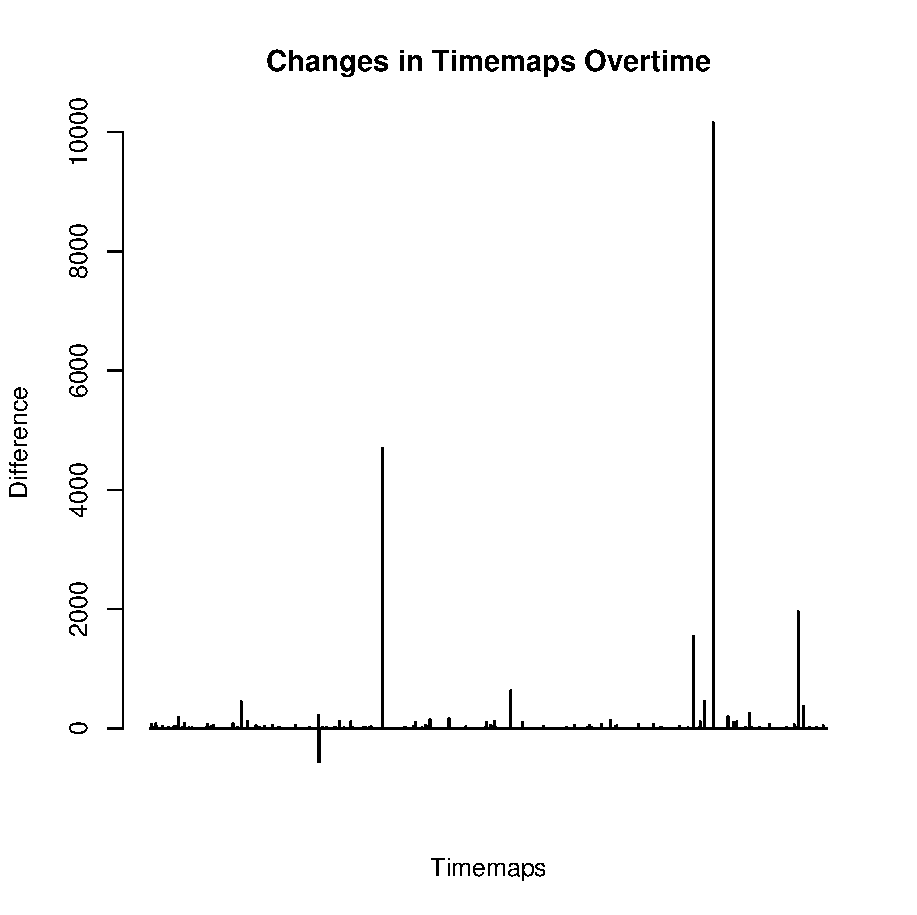
\includegraphics[scale=0.8]{timegraph.pdf}
 \caption{Bar graph for Timemap changes}
 \label{fig:q2split3}
 \end{figure}


\clearpage



% =================================
% Bibliography
% =================================

\begin{thebibliography}{9}
\bibitem{gitref}
cmuth001/anwala.github.io. ``GitHub''  N.p., May 01, 2018.\url{https://github.com/cmuth001/anwala.github.io/blob/master/Assignments/A7/blogdata.txt}
\bibitem{numref}
arthur-e/Programming-Collective-Intelligence. ``GitHub''. Web. May 01, 2018. \url{https://github.com/arthur-e/Programming-Collective-Intelligence/blob/master/chapter8/numpredict.py}
\bibitem{libref}
Cosine Similarity between 2 Number Lists``python - Cosine Similarity between 2 Number Lists - Stack Overflow''. n.p., n.d. Web. May 01, 2018. \url{https://stackoverflow.com/questions/18424228/cosine-similarity-between-2-number-lists}
\bibitem{gittingref}
Hrishi29/anwala.github.io. ``GitHub''  N.p., May 01, 2018.\url{https://github.com/Hrishi29/anwala.github.io/tree/master/Assignments/A2}

\end{thebibliography}

\end{document}